\begin{figure*}[htp!]
  \centering
  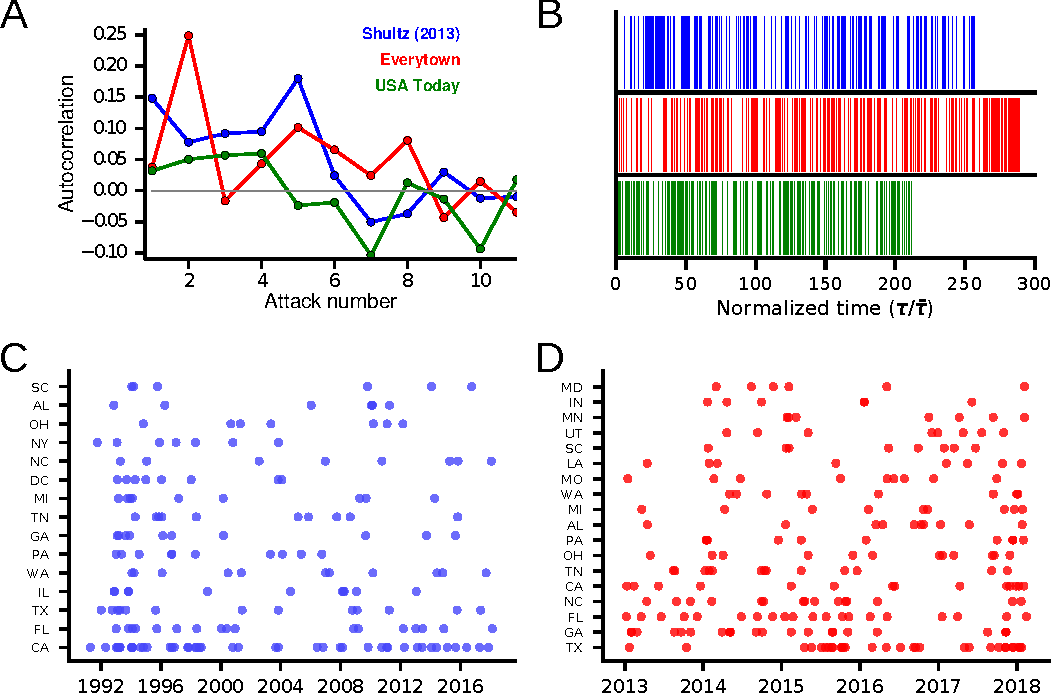
\includegraphics[width=0.9\textwidth]{S_clustering-optimized.pdf}
  \caption{       
    (A) Autocorrelation ($AC_f(n) = \frac{1}{N-n}
    \sum_{t=0}^{N-n-1}{f(t+n)f(t)}$) for the interevent time series
    ($f$) for the Shultz, Everytown and USA Today databases at
    different lags ($n$). The interevent time series has been
    normalized by substracting the mean and dividing by the standard
    deviation.
    (B) Attack series using the normalized interevent time. Vertical
    bars correspond to individual attacks.
    (C) Attack series by state in the Shultz dataset.
    (D) Attack series in the 8 towns with two or more attacks in the Everytown dataset.
  }
  \label{fig:S_clustering}
\end{figure*}
        
\begin{figure*}[htp!]
  \centering
  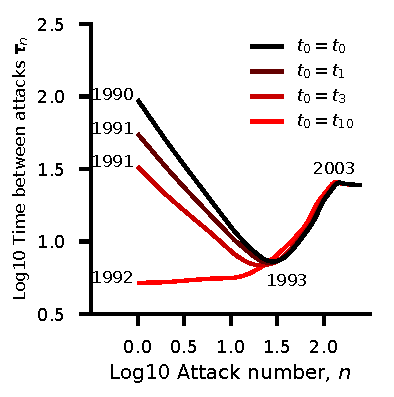
\includegraphics[width=0.495\textwidth]{S_redblue_sensitivity-optimized.pdf}
  \caption{
    The progress plot $\log_{10}{n}$ vs. $\log_{10}{\tau_n}$,
    using all attacks ($[0-n]$), attacks $[1-n]$, $[3-n]$ and
    $[10-n]$ in the Shultz database.
  } 
  \label{fig:S_redblue_sensitivity}
\end{figure*}

        
\begin{figure*}[htp!]
  \centering
  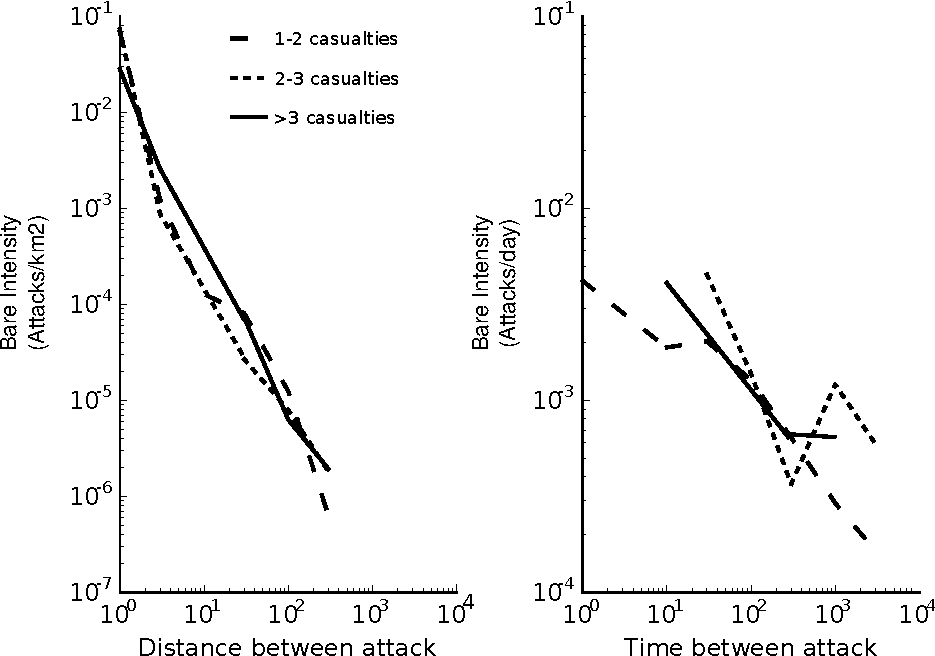
\includegraphics[width=0.495\textwidth]{S_magnitudeSparse-optimized.pdf}
  \caption{
    Kernel function of the Hawkes process by magnitude
    of attack. Intensity of attacks with respect to
    (left) distance between attacks and (right) time
    between attacks.
  }
  \label{fig:S_magnitudeSparse}
\end{figure*}
        
\begin{figure*}[ht!]
  \centering
  \includegraphics[width=0.9\textwidth]{S_hawkes_allAttacks-optimized.pdf}
  \caption{  
    (A) Fraction of attacks within a distance of each other, two null
    models where the attacks are drawn with probabily equal to the
    underlying US population and at times equal to the Schulz database
    (null model Shultz) or with frequency following a Poisson process
    (null model Poisson), and another null model where the attacks are
    drawn from the US area at random and at times equal to the Schulz
    database.
    (B) Intensity of attacks with respect to distance between attacks.  
    (C) Intensity of attacks with respect to time between attacks.
  }
  \label{fig:S_Hawkes}
\end{figure*}

\begin{figure*}[ht!]
  \centering
  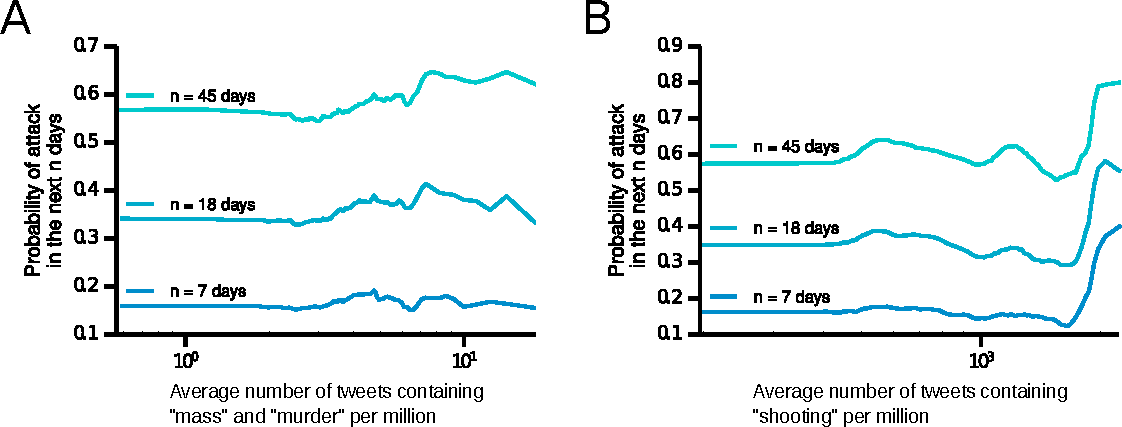
\includegraphics[width=0.9\textwidth]{S_copycat_otherWords-optimized.pdf}
  \caption{
    Probability of an attack happening in the 7, 18 or 45 days
    following attack $n$, as a function of the mean number of tweets
    with the words (A) ``mass'' and ``murder'' and (B) ``shooting" at
    days $n$ and ${n+1}$. The Shultz database was used for all plots.
  }
  \label{fig:S_copycat_otherWords}
\end{figure*}

\begin{figure*}[ht!]
  \centering
  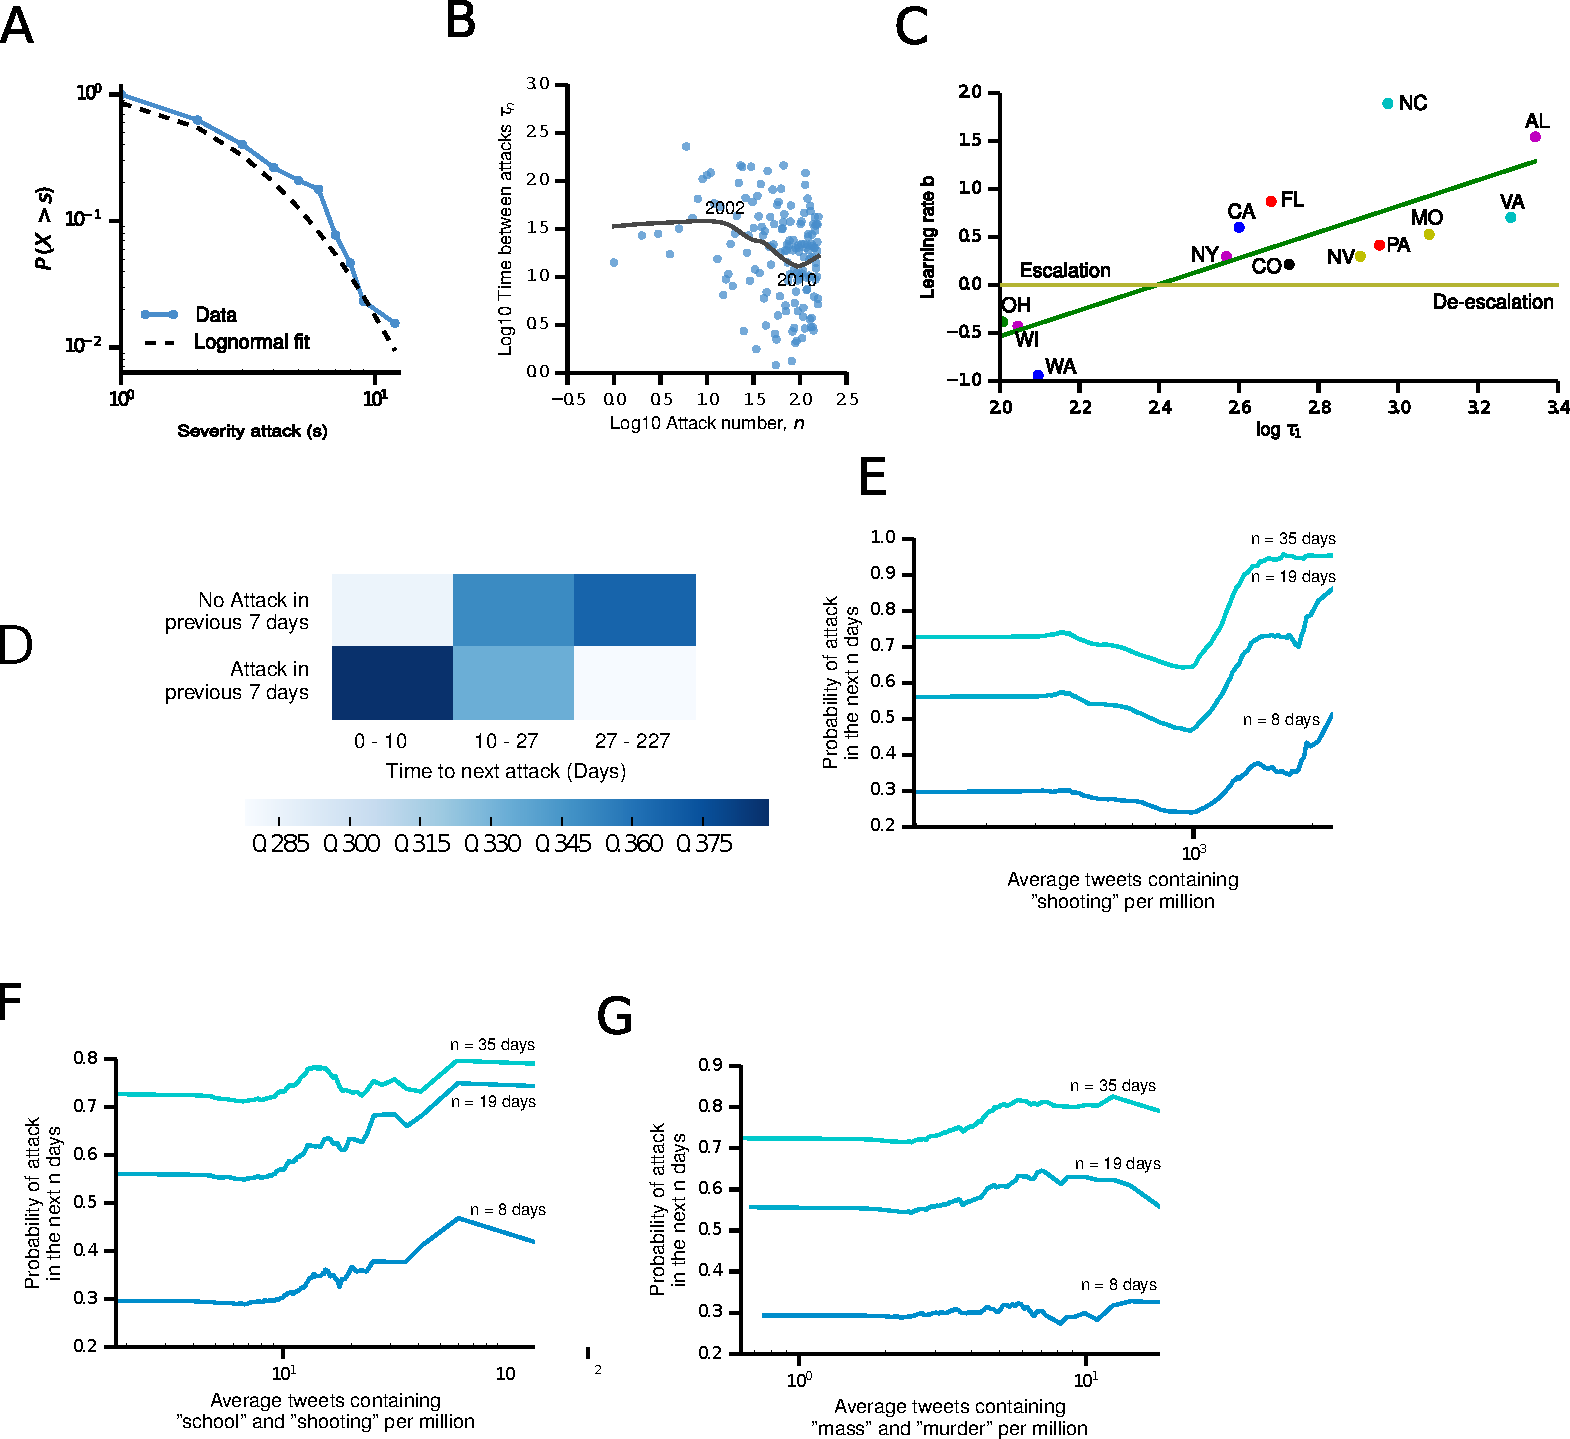
\includegraphics[width=0.9\textwidth]{S_FBIa-optimized.pdf}
  \caption{
    \textbf{Active shooting a} 
    (A) Complementary Cumulative Distribution Function (CCDF) for
    event severity (blue dots and solid line) and best fit (dashed
    line) to lognormal distribution.
    (B) The progress curve,
    $\log_{10}{n}$ vs. $\log_{10}{\tau_n}$, for all attacks. LOWESS
    fit ($\delta = 0$, $\alpha = 0.66$) is shown in dark gray, with
    the years where the trend changes annotated.
    (C) Prediction plot,
    $\log_{10}{\tau_1}$ vs. $b$. All states with more than four events
    are considered. States above the $b=0$ line experienced an
    escalation in the number of attacks.
    (D) Probability of attack
    depending on the presence of an attack in the previous seven
    days. Every bin contains one third of the attacks.
    (E--G) Probability of an attack happening in the 8, 19 or 35
    days following to attack $n$, as a function of the mean
    number of tweets talking about shootings at days $n$ and
    ${n+1}$.
  }
  \label{fig:S_FBIa}
\end{figure*}


\begin{figure*}[ht!]
  \centering
  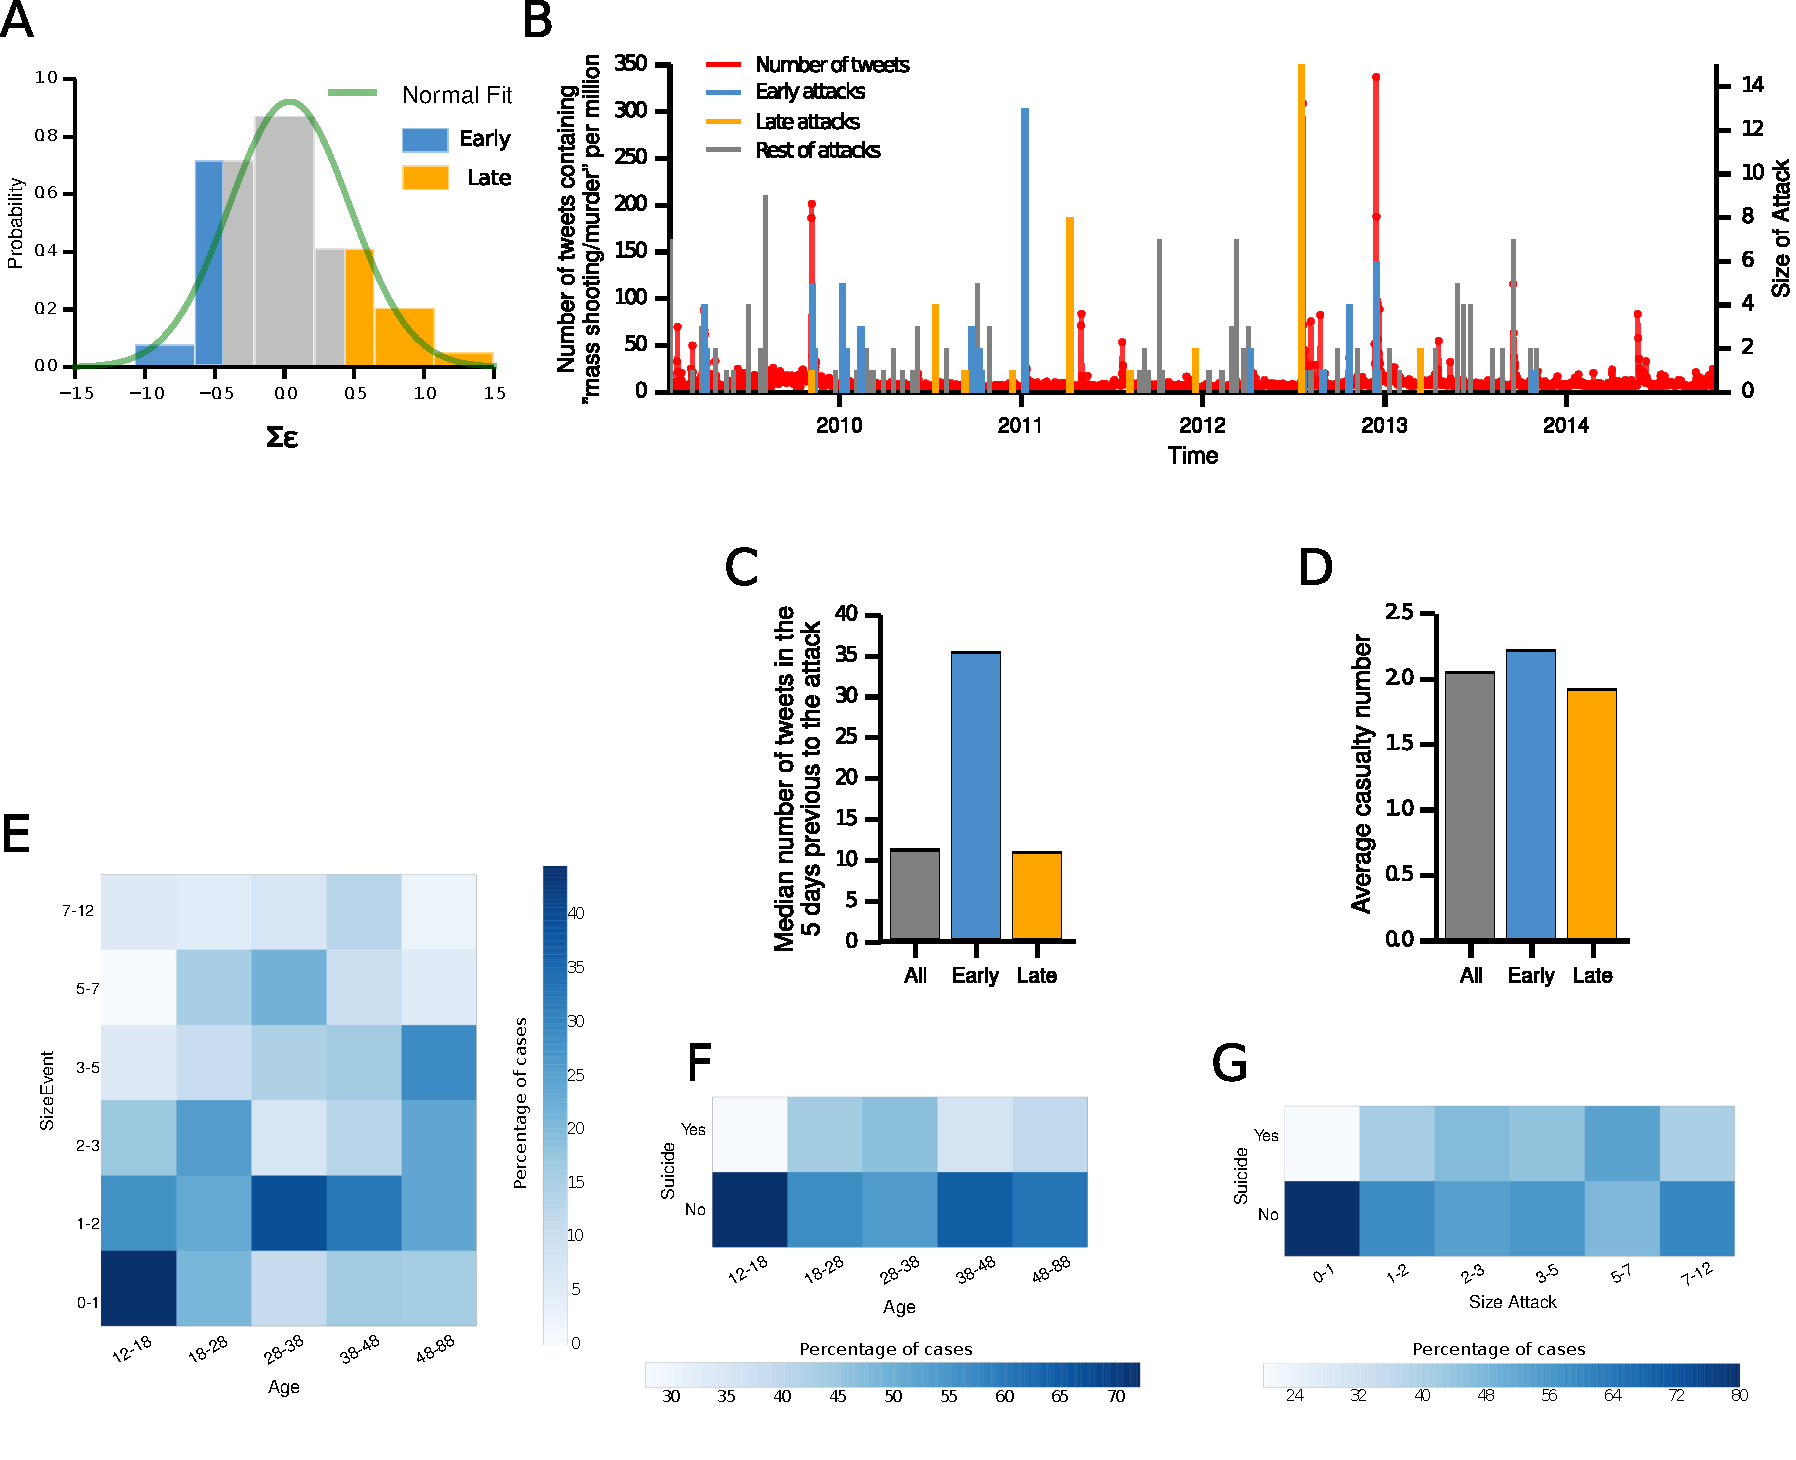
\includegraphics[width=0.9\textwidth]{S_FBIb-optimized.pdf}
  \caption{
    \textbf{Active shooting b}  
    (A) Histogram showing $\sum{\epsilon_j}$. \textit{Early} and
    \textit{Late} attacks are marked in blue and orange, respectively.
    (B) Time Series of the number of tweets containing ``mass'' and
    ``shooting'' or ``murder'' (Red lines, left axis), and the size of
    attacks (right axis) for \textit{Early} attacks (Blue),
    \textit{Late} attacks (Orange) and the rest (Grey).
    (C) Median number of tweets in the five days preceding All (Grey),
    \textit{Early} (Blue) and \textit{Late} (Orange) attacks.
    (D) Average casualty number for All (Grey), \textit{Early} (Blue) and
    \textit{Late} (Orange) attacks.
    (E) Probability of different magnitude of events by age group.
    (F) Probability of suicide by age group.
    (G) Probability of suicide by size of attack group.
  }
  \label{fig:S_FBIb}
\end{figure*}

